%==================================
\subsection{{\sc mixmod} function}
%==================================
The functions {\em mixmod.sci} and {\em mixmod.m} (Scilab and Matlab) are
available in the directory MIXMOD/.


{\noindent Remark With Scilab, you have to execute {\em initMixmod.sci} and with Matlab,
you have to add {\sc MIXMOD} and {\sc MIXMOD/UTIL/MATLAB} directories to Matlab path to load
{\sc MIXMOD} toolkit functions.}


%After executing {\em initMixmod.sci} in Scilab, or
%adding {\em mixmod path}
%in Matlab, {\em mixmod} functions can be used alone in a Scilab (or Matlab) program.

The calling sequence is
\begin{itemize}
%{\scriptsize
 \item quantitative case
{\scriptsize
\begin{verbatim}
-> (>>) [output [,outTab, optionalOutput]] = mixmod(data, nbCluster [,'criterion',criterion,
        'model',model,'weight', weight,'strategy',strategy,'partition',partition])

\end{verbatim}
}

%{\scriptsize
% \item quantitative case with HD models
%{\scriptsize
%\begin{verbatim}
%-> (>>) [output [,outTab, optionalOutput]] = mixmod(data, nbCluster [,'criterion',criterion,
%        'model',model,'weight', weight,'strategy',strategy,'partition',partition,
%        'subDimension',subDimension])
%
%\end{verbatim}
%





%{\scriptsize
\item qualitative case
% {\tiny
{\scriptsize
 \begin{verbatim}
 -> (>>) [output [,outTab, optionalOutput]] = mixmod(data, nbCluster, 'tabModality',tabModality
         [,'criterion',criterion,'model',model,'weight',weight,'strategy',strategy,'partition',partition])

 \end{verbatim}
 }
\end{itemize}

%{\it Warning
%In the quantitative case, the option subDimension,
%have to be used in a discriminant analysis situation and with the HD models (cf. Table \ref{16models}).}

\vspace*{0.5cm}

In the following examples, we will either consider quantitative or qualitative data sets. The quantitative data set will
be named {\it geyser} and the qualitative one {\it b\_toby}.\\

The principal differences between qualitative and quantitative treatement is the presence of the variable 'tabModality'
in the qualitative case.
%-------------------------------------------
%-------------------------------------------
\subsubsection{Begining with {\sc mixmod}}

The simplest way (without options) to execute {\sc mixmod} function is
%-------------------------------------------
%-------------------------------------------


\begin{tabular}{c|c}
\begin{minipage}[c]{0.40\columnwidth}%
{\scriptsize
\begin{verbatim}
    -> geyser = read('DATA/geyser.dat',272,2);

    -> b_toby = read('DATA/b_toby.dat',216,4);
\end{verbatim}}
\end{minipage}%
&
\begin{minipage}[c]{0.60\columnwidth}%
{\scriptsize
\begin{verbatim}
    >> geyser = load('DATA/geyser.dat');

    >> b_toby = load('DATA/b_toby.dat');
\end{verbatim}}
\end{minipage}%
\end{tabular}


{\scriptsize
\begin{verbatim}
      -> (>>) nbCluster1 = 2;
      -> (>>) tabModality = [2 ; 2 ; 2 ; 2];
      -> (>>) out1 = mixmod(b_toby, nbCluster1,'tabModality',tabModality);
      -> (>>) nbCluster2 = [2; 3];
      -> (>>) out2 = mixmod(geyser, nbCluster2);

\end{verbatim}}

%\end{enumerate}


%-------------------------------------------
%-------------------------------------------
\subsubsection{Executing {\sc mixmod} with options}


\begin{itemize}

\item criterion a vector of strings (scilab) or a cell array of strings (matlab)


\begin{tabular}{c|c}
\begin{minipage}[c]{0.47\columnwidth}%
{\scriptsize
\begin{verbatim}
    -> criterion = 'BIC';
    -> out = mixmod(geyser, 2, 'criterion',criterion);
    -> criteria = ['BIC'; 'ICL'; 'NEC'];
    -> out = mixmod(geyser, 2 ,'criterion',criteria);

\end{verbatim}}
\end{minipage}%
&
\begin{minipage}[c]{0.58\columnwidth}%
{\scriptsize
\begin{verbatim}
    >> criterion = 'BIC';
    >> out = mixmod(geyser, 2, 'criterion',criterion);
    >> criteria = {'BIC'; 'ICL'; 'NEC'};
    >> out = mixmod(geyser, 2, 'criterion',criteria);

\end{verbatim}}
\end{minipage}%
\end{tabular}



\item models a structure containing three fields name, subDimensionFree, subDimensionEqual defining the caracteristics
      of a model.
%vector of strings (scilab) or cell array of strings (matlab)



\begin{tabular}{c|c}
\begin{minipage}[c]{0.5\columnwidth}%
{\scriptsize
\begin{verbatim}
    -> model = tlist(['model','name','subDimensionFree',
               'subDimensionEqual'],'',[],[]);
    -> model.name = 'Binary_pk_Ekj';
    -> out = mixmod(b_toby,2,'tabModality',tabModality,
                   'model',list(model));

    -> model1 = tlist(['model','name','subDimensionFree',
               'subDimensionEqual'],'Binary_pk_Ek',[],[]);
    -> model2 = tlist(['model','name','subDimensionFree',
               'subDimensionEqual'],'Binary_pk_Ej',[],[]);
    -> model3 = tlist(['model','name','subDimensionFree',
               'subDimensionEqual'],'Binary_pk_E',[],[]);
    -> models = list(model1,model2,model3);
    -> out = mixmod(b_toby,2,'tabModality',tabModality,
                   'model',models);

\end{verbatim}}
\end{minipage}%
&
\begin{minipage}[c]{0.58\columnwidth}%
{\scriptsize
\begin{verbatim}
  >> model = struct('name','','subDimensionFree',
               [],'subDimensionEqual',[]);
  >> model.name = 'Binary_pk_Ekj';
  >> out = mixmod(b_toby, 2, 'tabModality',tabModality,
                   'model',{model});
  >> model1 = struct('name','Binary_pk_Ek','subDimensionFree',
               [],'subDimensionEqual',[]);
  >> model2 = struct('name','Binary_pk_Ej','subDimensionFree',
              [],'subDimensionEqual',[]);
  >> model3 = struct('name','Binary_pk_E','subDimensionFree',
               [],'subDimensionEqual',[]);
  >> models = {model1,model2,model3};
  >> out = mixmod(b_toby, 2, 'tabModality',tabModality,
                    'model',models);

\end{verbatim}}
\end{minipage}%
\end{tabular}



\item weight a vector of real or integer values (scilab and matlab)


\begin{tabular}{c|c}
\begin{minipage}[c]{0.52\columnwidth}%
{\scriptsize
\begin{verbatim}

    -> weight = read('DATA/b_toby.wgt',216,1);
    -> out    = mixmod(b_toby, 2, 'tabModality',tabModality,
                       'weight',weight);

\end{verbatim}}
\end{minipage}%
&
\begin{minipage}[c]{0.52\columnwidth}%
{\scriptsize
\begin{verbatim}
 >> weight = load('DATA/b_toby.wgt');
 >> out    = mixmod(b_toby, 2, 'tabModality',tabModality,
                       'weight',weight);

\end{verbatim}}
\end{minipage}%
\end{tabular}


\item partition a list of partition matrices (scilab) or a cell array of partition matrices (matlab)


\begin{tabular}{c|c}
\begin{minipage}[c]{0.52\columnwidth}%
{\scriptsize
\begin{verbatim}

    -> part2 = read('DATA/geyser.part',272,2);
    -> out = mixmod(geyser, 2, 'partition',list(part2));

    -> part3 = read('DATA/geyser3clusters.part',272,3);
    -> out = mixmod(geyser, [2;3], 'partition',
             list(part2, part3));
\end{verbatim}}
\end{minipage}
&
\begin{minipage}[c]{0.51\columnwidth}
{\scriptsize
\begin{verbatim}

    >> part2 = load('DATA/geyser.part');
    >> out = mixmod(geyser, 2, 'partition',{part2});

    >> part3 = load('DATA/geyser3clusters.part');
    >> out = mixmod(geyser, [2;3], 'partition',
            {part2; part3});
\end{verbatim}}
\end{minipage}
\end{tabular}



\item strategies a structure or a list of structures containing two fields, the first one
defining the way of initializing
the strategy ({\it initialization}) and the second the algorithms that can be used ({\it algorithm}).

\begin{itemize}
\item strategies initialization type a structure (scilab and matlab)


	\begin{tabular}{c|c}
	\begin{minipage}[c]{0.47\columnwidth}%
{\scriptsize
	\begin{verbatim}

-> init1  = tlist(['initialization','name','param',
     'partition'],'SMALL_EM',list(),list());

\end{verbatim}}
	\end{minipage}%
&
	\begin{minipage}[c]{0.58\columnwidth}%
{\scriptsize
	\begin{verbatim}

>>  init1 = struct('name','SMALL_EM','param',
       [],'partition',{{}});

\end{verbatim}}
	\end{minipage}%
	\end{tabular}\\



	\begin{tabular}{c|c}
	\begin{minipage}[c]{0.47\columnwidth}%
{\scriptsize
	\begin{verbatim}

-> init2 = tlist(['initialization','name','param',
     'partition'],'USER',list(),list());
-> init2.param = out.modelOutput(1).param;

\end{verbatim}}
	\end{minipage}%
&
	\begin{minipage}[c]{0.58\columnwidth}%
{\scriptsize
	\begin{verbatim}

>> init2 = struct('name','USER','param',
     [],'partition',{{}});
>> init2.param = out.modelOutput.param;

\end{verbatim}}
	\end{minipage}%
	\end{tabular}\\



\begin{tabular}{c|c}
	\begin{minipage}[c]{0.47\columnwidth}%
	{\scriptsize
	\begin{verbatim}

-> init3  = tlist(['initialization','name','param',
    'partition'],'USER_PARTITION',list(),list());
-> p2 = read('DATA/geyser.part',272,2);
-> p3 = read('DATA/geyser3clusters.part',272,3);
-> init3.partition = list(p2, p3);

\end{verbatim}}
	\end{minipage}%
&
	\begin{minipage}[c]{0.58\columnwidth}%
	{\scriptsize
	\begin{verbatim}

>> init3 = struct('name','USER_PARTITION','param',
     [],'partition',{{}});
>> p2 = load('DATA/geyser.part');
>> p3 = load('DATA/geyser3clusters.part');
>> init3.partition = {p2, p3};

\end{verbatim}}
	\end{minipage}%
	\end{tabular}\\






\item strategies algorithms type a structure (scilab and matlab)



	\begin{tabular}{c|c}
	\begin{minipage}[c]{0.42\columnwidth}%
	{\scriptsize
	\begin{verbatim}

-> algo1 = tlist(['algorithm','name','stopRule',
    'stopRuleValue'],'EM','EPSILON',0.0001);
-> algo2 = tlist(['algorithm','name','stopRule',
     'stopRuleValue'],'CEM',
     'NBITERATION_EPSILON',[100; 0.0001]);

\end{verbatim}}
	\end{minipage}%
&
	\begin{minipage}[c]{0.58\columnwidth}%
	{\scriptsize
	\begin{verbatim}

>> algo1 = struct('name','EM','stopRule',{'EPSILON'},
    'stopRuleValue',[0.0001]);
>> algo2 = struct('name','CEM','stopRule',
   'NBITERATION_EPSILON',
   'stopRuleValue',[100 ; 0.0001]);

\end{verbatim}}
	\end{minipage}%
	\end{tabular}\\

%---------------------------------------------------------
	\item{strategy example }
%---------------------------------------------------------


\begin{tabular}{c|c}
\begin{minipage}[c]{0.46\columnwidth}%
{\scriptsize
\begin{verbatim}

-> init1 = tlist(['initialization','name','param',
    'partition'],'SMALL_EM',list(),list());
-> algo1 = tlist(['algorithm','name','stopRule',
    'stopRuleValue'],'EM','EPSILON',0.0001);
-> algo2 = tlist(['algorithm','name','stopRule',
    'stopRuleValue'],'CEM',
    'NBITERATION_EPSILON',[100; 0.0001]);
-> algos = list(algo1,algo2);
-> strategy  = tlist(['strategyType','initialization',
    'algorithm'],init1,algos);
-> out = mixmod(b_toby, 2, 'tabModality',tabModality,
                'strategy',strategy);

\end{verbatim}}
\end{minipage}%
&
\begin{minipage}[c]{0.54\columnwidth}%
{\scriptsize
\begin{verbatim}

>> init1 = struct('name','SMALL_EM','param',
    [],'partition',{{}});
>> algo1 = struct('name','EM','stopRule',
    {'EPSILON'},'stopRuleValue',[0.0001]);
>> algo2 = struct('name','CEM','stopRule',
    'NBITERATION_EPSILON','stopRuleValue',
     [100 ; 0.0001]);
>> algos  = [algo1 ; algo2];
>> strategy = struct('initialization',init1,'algorithm',algos);
>> out = mixmod(b_toby, 2,'tabModality',tabModality,
                'strategy',strategy);

\end{verbatim}}
\end{minipage}%
\end{tabular}

\end{itemize}


\end{itemize}

%-------------------------------------------
%-------------------------------------------
\subsubsection{Output}
%-------------------------------------------
%-------------------------------------------
{\sc mixmod} functions return a required output structure {\em output} and two optional outputs {\em outTab} and {\em optionalOutput}.
%------------------------------------------------------
\paragraph{Output structure}
%------------------------------------------------------
A structure with two fields
\begin{itemize}
  \item condExe containing the conditions of execution of {\sc mixmod}.
%  \item modelOutput a list of modelOutput structures (scilab) or a vector of  modelOutput structures (matlab) (for each criterion) for the best configuration (among all models, strategies and number of clusters).

A structure with fifteen or sixteen fields
\begin{itemize}
  \item data the matrix $[n,d]$ of individuals ($n$ number of samples, $d$ number of variables) (see Section \ref{individualsRepresentationSection}),
	\item weight the vector of real or integer values defining the weight of the data,
	\item dataType an integer defining the type of the data set
                         (1 for gaussian data type and 2 for binary data type),
  \item nbSamples an integer representing the number of samples $n$,
  \item weightTotal a number representing the total weight,
  \item pbDimension an integer representing the problem dimension $d$ (number of variables),
  %\item subDimension a vector of integer or an integer representing the intrinsic dimension of each class,
   \item nbCluster a vector of integers representing the number of clusters,
  \item tabModality a vector of integers representing the modality of each variable in qualitative case,
  \item criterion a vector of strings (scilab) or a cell array of strings (matlab) defining the type of criterion(ia),
  \item modelType a list of model structures (scilab) or a cell array of model structures (matlab) defining the type
        of models,
  \item strategy a list of strategy structures (scilab) or a vector of strategy structures (matlab) defining the type of strategy(ies),
%	\item knownPartition a list of partition matrices (scilab) or a cell array of partition matrices (matlab) defining known partition for the data,
  \item mixmodError an integer representing the code error of mixmod execution (0 if mixmod runs successfully),
  \item tabEstimError a vector representing the code error of each configuration (combination of strategy, number of clusters and model) (0 if no error),
  \item tabCriterError a vector representing the code error in the criterion value calculation for each combination
  of strategy, number of clusters and model,
  \item tabSelecError a vector representing the code error of selections of the best configuration.
\end{itemize}

{\noindent Examples of access to fields}
{\scriptsize
\begin{verbatim}
    -> (>>) output.condExe
    -> (>>) output.condExe.nbSamples
    -> (>>) output.condExe.pbDimension
    -> (>>) output.condExe.nbCluster
    -> (>>) output.condExe.criterion
    -> (>>) output.condExe.modelType                  // (%) the first model (if several models)
    -> (>>) output.condExe.strategy(1).initialization.name     // (%) the first strategy (if several strategies)
\end{verbatim}}


\item modelOutput a list of outputs (scilab) or a vector of outputs (matlab) (for each criterion)
                    for the best configuration (among all models, strategies and number of clusters).

A structure with eight fields
\begin{itemize}
  \item type string giving the best model type,
  \item nbCluster integer giving the best number of clusters,
  \item criterion structure giving the name and the value of the criterion,
  \item strategy the best strategy structure,
  \item param structure giving the parameters of the best model, (proportions, means and dispersion or
    proportions, means, subDimension, parameters\_Akj, parameters\_Bk, orientation)
  \item proba (only if standard output) structure giving the labels, the partition and the posterior probabilities
                 of the best model,
  \item likelihood (only if standard output) structure giving the loglikelihood, the complete loglikelihood,
                     the number of free parameters and the entropy for the best model.
  \item error the code error of the model.
\end{itemize}

Note in the quantitative case, the dispersion represents the variance matrix.\\

\vspace*{0.5cm}
{\noindent Examples of access to fields}
{\scriptsize
\begin{verbatim}
    -> (>>) output.modelOutput(1).type       // % for the 1st criterion
    -> (>>) output.modelOutput(1).criterion  // % for the 1st criterion
    -> (>>) output.modelOutput(1).param
\end{verbatim}}


{\scriptsize
\begin{verbatim}
    -> (>>) output.modelOutput(1).criterion.name
    -> (>>) output.modelOutput(1).criterion.value
    -> (>>) output.modelOutput(1).nbCluster
    -> (>>) output.modelOutput(1).param.proportion
    -> (>>) output.modelOutput(1).param.mean
    -> (>>) dis = output.modelOutput(1).param.dispersion
\end{verbatim}}






\begin{tabular}{c|c}
 \begin{minipage}[c]{0.46 \columnwidth} %
  {\scriptsize
    \begin{verbatim}
 -> dis(1) // (%) variance of first mixture component
 -> dis(2)// (%) variance of second mixture component
    \end{verbatim}
 }
    \end{minipage} %
&
\begin{minipage}[c]{0.54 \columnwidth} %
 {\scriptsize
   \begin{verbatim}
>> dis{1} // (%) variance of first mixture component
>> dis{2} // (%) variance of second mixture component
   \end{verbatim}
 }
   \end{minipage} %

\end{tabular}



{\scriptsize
\begin{verbatim}
    -> (>>) output.modelOutput(1).proba.label
    -> (>>) output.modelOutput(1).proba.partition
    -> (>>) output.modelOutput(1).proba.postProba
\end{verbatim}}

{\scriptsize
\begin{verbatim}
    -> (>>) output.modelOutput(1).likelihood.logLikelihood
    -> (>>) output.modelOutput(1).likelihood.completeLL
    -> (>>) output.modelOutput(1).likelihood.nbFreeParam
    -> (>>) output.modelOutput(1).likelihood.entropy
\end{verbatim}}


\end{itemize}


%-------------------------------------------
%-------------------------------------------
\subsubsection{Optional output}
%-------------------------------------------
%-------------------------------------------
Two optional outputs are available
\begin{itemize}
  \item {\em outTab} a four dimension matrix which contains values of all criteria for all estimations (chosen by
  the user) all combinations of strategies, numbers of different cluster members and models.
  The first dimension represents strategies, the second the number of clusters, the third represents models and the
  last, criteria.\\
	\vspace{1cm}\\
  Example of using

\begin{tabular}{c|c}
\begin{minipage}[c]{0.53\columnwidth}%
{\scriptsize
\begin{verbatim}
    -> nbCluster = [2; 3; 4];
    -> criteria  = ['BIC'; 'ICL'];
    -> model1 = tlist(['model','name','subDimensionFree',
                'subDimensionEqual'],'Gaussian_p_L_I',[],[]);
    -> model2 = tlist(['model','name','subDimensionFree',
                'subDimensionEqual'],'Gaussian_p_Lk_I',[],[]);
    -> model3 = tlist(['model','name','subDimensionFree',
                'subDimensionEqual'],'Gaussian_pk_L_I',[],[]);
    -> model4 = tlist(['model','name','subDimensionFree',
               'subDimensionEqual'],'Gaussian_pk_Lk_I',[],[]);
    -> models    = list(model1,model2,model3,model4);
\end{verbatim}}
\end{minipage}%
&
\begin{minipage}[c]{0.47\columnwidth}%
{\scriptsize
\begin{verbatim}
 >> nbCluster = [2; 3; 4];
 >> criteria  = {'BIC'; 'ICL'};
 >> model1 = struct('name','Gaussian_p_L_I','subDimensionFree',
                [],'subDimensionEqual',[]);
 >> model2 = struct('name','Gaussian_p_Lk_I','subDimensionFree',
                [],'subDimensionEqual',[]);
 >> model3 = struct('name','Gaussian_pk_L_I','subDimensionFree',
                [],'subDimensionEqual',[]);
 >> model4 = struct('name','Gaussian_pk_Lk_I','subDimensionFree',
                [],'subDimensionEqual',[]);
 >> models    = {model1,model2,model3,model4};
\end{verbatim}}
\end{minipage}%
\end{tabular}
{\scriptsize
\begin{verbatim}
    -> (>>) [out, outTab, optionalOutput] = mixmod(geyser, nbCluster, 'criterion',criteria, 'model',models);
\end{verbatim}}

{\scriptsize
\begin{verbatim}
    -> (>>) value = outTab(1, 2, 1, 1);
\end{verbatim}}
\vspace{-0.4cm}
This command returns the first criterion (BIC) value for the first strategy (default strategy), the second number
of clusters (3) and the first model (Gaussian\_p\_L\_I).\\

{\scriptsize
\begin{verbatim}
    -> (>>) value = outTab(1, 1, 4, 2);
\end{verbatim}}
\vspace{-0.4cm}
This command returns the second criterion (ICL) value for the first strategy (default strategy), the first number
of clusters (2) and the fourth model (Gaussian\_pk\_Lk\_I).\\

{\scriptsize
\begin{verbatim}
    -> (>>) value = outTab(1,,:,:);
\end{verbatim}}
\vspace{-0.4cm}
This command returns all criterion (BIC, ICL) values for the first strategy (default strategy), all
number of clusters (2, 3, 4) and all models (24 values).\\


  \item {\em optionalOutput}: it is the same output as {\em output} but for all configurations (or estimations) (an estimation or configuration is a combination of a number of cluster, a model type and a strategy) except for the following fields:
\begin{itemize}
  \item criterion: The field criterion of {\em modelOutput} structure regroups informations about each criterion.
  \item proba: empty.
  \item likelihood: empty.
\end{itemize}

Note: Number of estimation = number of number of clusters * number of models * number of strategies.

\begin{tabular}{c|c}
\begin{minipage}[c]{0.48\columnwidth}%
{\scriptsize
\begin{verbatim}

-> nbCluster = [2; 3; 4];
-> criteria  = ['BIC'; 'ICL'];
-> model1 = tlist(['model','name','subDimensionFree',
          'subDimensionEqual'],'Gaussian_p_L_I',[],[]);
-> model2 = tlist(['model','name','subDimensionFree',
          'subDimensionEqual'],'Gaussian_p_Lk_I',[],[]);
-> model3 = tlist(['model','name','subDimensionFree',
          'subDimensionEqual'],'Gaussian_pk_L_I',[],[]);
-> model4 = tlist(['model','name','subDimensionFree',
          'subDimensionEqual'],'Gaussian_pk_Lk_I',[],[]);
-> models    = list(model1,model2,model3,model4);

\end{verbatim}}
\end{minipage}%
&
\begin{minipage}[c]{0.5\columnwidth}%
{\scriptsize
\begin{verbatim}

>> nbCluster = [2; 3; 4];
>> criteria  = {'BIC'; 'ICL'};
>> model1 = struct('name','Gaussian_p_L_I','subDimensionFree',
               [],'subDimensionEqual',[]);
>> model2 = struct('name','Gaussian_p_Lk_I','subDimensionFree',
               [],'subDimensionEqual',[]);
>> model3 = struct('name','Gaussian_pk_L_I','subDimensionFree',
               [],'subDimensionEqual',[]);
>> model4 = struct('name','Gaussian_pk_Lk_I','subDimensionFree',
              [],'subDimensionEqual',[]);
>> models    = {model1,model2,model3,model4};


\end{verbatim}}
\end{minipage}%
\end{tabular}
{\scriptsize
\begin{verbatim}
    -> (>>) [out, outTab, optionalOutput] = mixmod(geyser, nbCluster,'criterion',criteria,'model',models);
    -> (>>) optionalOutput.condExe
    -> (>>) optionalOutput.modelOutput(2).type
    -> (>>) optionalOutput.modelOutput(12).param
\end{verbatim}}

In this case, there are twelve estimations for each criterion.
\end{itemize}


%-------------------------------------------
%-------------------------------------------
\subsubsection{Examples}
%-------------------------------------------
%-------------------------------------------
Examples are written if MIXMOD/ directory is the current directory.
\begin{itemize}
	\item Scilab quantitative examples\\



{\scriptsize
\begin{verbatim}

data       = read('DATA/geyser.dat',272,2);
criterion  = ['BIC' ; 'ICL'];
model1 = tlist(['model','name','subDimensionFree','subDimensionEqual'],'Gaussian_p_L_I',[],[]);
model2 = tlist(['model','name','subDimensionFree','subDimensionEqual'],'Gaussian_p_Lk_I',[],[]);
model3 = tlist(['model','name','subDimensionFree','subDimensionEqual'],'Gaussian_pk_L_I',[],[]);
model4 = tlist(['model','name','subDimensionFree','subDimensionEqual'],'Gaussian_pk_Lk_I',[],[]);
model    = list(model1,model2,model3,model4);

weight     = read('DATA/geyser.wgt',272,1);

init  = tlist(['initialization','name','param','partition'],'SMALL_EM',list(),list());
algo1     = tlist(['algorithm','name','stopRule','stopRuleValue'],'EM','EPSILON',0.0001);
algo2     = tlist(['algorithm','name','stopRule','stopRuleValue'],'CEM','NBITERATION_EPSILON',[100 0.0001]);
algo   = list(algo1,algo2);
strategy  = tlist(['strategyType','initialization','algorithm'],init,algo);
output = mixmod(data,2);
output = mixmod(data,2,'weight',weight);
output = mixmod(data,[2;3],'criterion',criterion,'model',model,'strategy',strategy);
[output, outTab] = mixmod(data,[2;3],'model',model);
[output, outTab, optionalOutput] = mixmod(data,2,'criterion',criterion,'strategy',strategy,'weight',weight);

output = mixmod(data,2);
geyserPart2Clusters = output.modelOutput(1).proba.partition;
strategy.initialization.name = 'USER_PARTITION';
strategy.initialization.partition = list(geyserPart2Clusters);
output = mixmod(data,2,'strategy',strategy);

output = mixmod(data,2);
geyserPart2Clusters = output.modelOutput(1).proba.partition;
geyserPart3Clusters=zeros(272,3);
geyserPart3Clusters(1:100,1)=1;
geyserPart3Clusters(101:200,2)=1;
geyserPart3Clusters(201:272,3)=1;
strategy.initialization.partition = list(geyserPart2Clusters, geyserPart3Clusters);
output = mixmod(data,[2;3],'strategy',strategy);

output = mixmod(data,2);
strategy.initialization.name = 'USER';
strategy.initialization.param = list(output.modelOutput(1).param);
output = mixmod(data,2,'criterion',criterion,'model',model,'strategy',strategy);


// Using USER initialization


[criterion,strategy] = mixmodInputStrategy();

u=file('open','DATA/geyser.init','old');

nbCluster = 2;
pbDimension = 2;

proportion = [];
meand = list();
vard = list();
scatter = [];
for k=1:nbCluster
   proportion = [proportion read(u,1,1)];
   meand(k) = [];
   meand(k) = [read(u,1,pbDimension)];
   vard(k) = [];
   vard(k) = read(u,pbDimension,pbDimension);
end;

file('close',u);

tabParam = list(tlist(['parameterType','proportion','mean','dispersion'],proportion,meand,vard));
strategy.initialization.param = tabParam;

output = mixmod(data,3,'strategy',strategy);
\end{verbatim}

{\normalsize \textbf{Example for discriminant analysis (in directory MIXMOD/)}:}

\begin{verbatim}

//Step 1:
dataTraining = read('DATA/geyser.dat',272,2);
partition    = read('DATA/geyser.part',272,2);
[criterion1,strategy1] = mixmodInputStrategy('DAstep1');
//Press Enter in Scilab

strategy1.initialization.partition = list(partition);
model = tlist(['model','name','subDimensionFree','subDimensionEqual'],'Gaussian_p_L_I',[],[]);
output = mixmod(dataTraining,2,'criterion',criterion1,'model',list(model),'strategy',strategy1,
        'partition',list(partition));
//Step 2:
[criterion2,strategy2] = mixmodInputStrategy('DAstep2');
//Press Enter in Scilab

strategy2.initialization.param = list(output.modelOutput(1).param);
dataRemaining = read('DATA/geyser.discriminant.dat',5,2);
output2 = mixmod(dataRemaining,2,'criterion',criterion2,'model',list(model),'strategy',strategy2);
\end{verbatim}

{\normalsize \textbf{Example for discriminant analysis with HD models} }

\begin{verbatim}

dataTraining = read('DATA/crabes.dat',200,5);
partition    = read('DATA/crabes.part',200,4);
model1 = tlist(['model','name','subDimensionFree','subDimensionEqual'],'Gaussian_HD_pk_AkjBkQkD'
          ,[],[2;3]);
model2 = tlist(['model','name','subDimensionFree','subDimensionEqual'],'Gaussian_HD_pk_AkjBkQkDk'
         ,[1,2,2,1;2,1,1,2],[]);
model = list(model1,model2);
[criterion1,strategy1] = mixmodInputStrategy('DAstep1');
//Press Enter in Scilab

strategy1.initialization.partition = list(partition);
output = mixmod(dataTraining,4,'criterion',criterion1,'model',model,'strategy',strategy1,'partition'
         ,list(partition));

//Step 2:
bestModel = output.modelOutput(1).type;
[criterion2,strategy2] = mixmodInputStrategy('DAstep2');
//Press Enter in Scilab

strategy2.initialization.param = list(output.modelOutput(1).param);
dataRemaining = read('DATA/crabes_10indiv.dat',10,5);
output2 = mixmod(dataRemaining,4,'criterion',criterion2,'model',list(bestModel),'strategy',strategy2);


\end{verbatim}}


\item Scilab qualitative examples \\
{\scriptsize

 \begin{verbatim}

data = read('DATA/birds.dat',153,6);
partition    = read('DATA/birds.part',153,3);
tabModality = [2 ; 4 ; 5 ; 2 ; 5 ; 3];
criterion = ['BIC','ICL', 'NEC'];

model1 = tlist(['model','name','subDimensionFree','subDimensionEqual'],'Binary_pk_Ekjh',[],[]);
model2 = tlist(['model','name','subDimensionFree','subDimensionEqual'],'Binary_pk_Ekj',[],[]);
model3 = tlist(['model','name','subDimensionFree','subDimensionEqual'],'Binary_pk_Ek',[],[]);
model4 = tlist(['model','name','subDimensionFree','subDimensionEqual'],'Binary_pk_Ej',[],[]);
model5 = tlist(['model','name','subDimensionFree','subDimensionEqual'],'Binary_pk_E',[],[]);
model    = list(model1,model2,model3,model4,model5);

weight    = read('DATA/birds.lab',153,1);

init1 = tlist(['initialization','name','param','partition'],'CEM_INIT',list(),list());
algo1 = tlist(['algorithm','name','stopRule','stopRuleValue'], 'EM', 'NBITERATION_EPSILON',[300,0.0001]);
algo2 = tlist(['algorithm','name','stopRule','stopRuleValue'], 'CEM', 'EPSILON',0.001);
strategy = tlist(['strategyType','initialization','algorithm'],init1,list(algo1, algo2));

output = mixmod(data,[2;3],'tabModality',tabModality);
output = mixmod(data,[2;3],'tabModality',tabModality,'criterion',criterion);
output = mixmod(data,2,'tabModality',tabModality,'strategy',strategy);
output = mixmod(data,2,'tabModality',tabModality,'weight',weight,'strategy',strategy);
output = mixmod(data,3,'tabModality',tabModality,'partition',list(partition));
[output,outTab] = mixmod(data,2,'tabModality',tabModality,'criterion',criterion,'model',model);

strategy.initialization.name = 'USER';
strategy.initialization.param = list(output.modelOutput(1).param);
out = mixmod(data,2,'tabModality',tabModality,'strategy',strategy);

mixmodView(out);
mixmodView(out, 'mca1D');
mixmodView(out, 'mca2D', 'pointClass');
mixmodView(out, 'mca3D', 'class');

mixmodView(out, [1],'point');
mixmodView(out, [1 2],'class');

  \end{verbatim}
{\normalsize \textbf {Example for discriminant analysis (in directory MIXMOD/):}}

 \begin{verbatim}

//Step 1:
dataTraining = read('DATA/b_toby.dat',216,4);
partition    = read('DATA/b_toby.part',216,2);
model = tlist(['model','name','subDimensionFree','subDimensionEqual'],'Binary_pk_Ekjh',[],[]);
tabModality = [2;2;2;2];
[criterion1,strategy1] = mixmodInputStrategy('DAstep1');
//Press Enter in Scilab

strategy1.initialization.partition = list(partition);
output = mixmod(dataTraining,2,'tabModality',tabModality,'criterion',criterion1,'model',list(model),'strategy'
,strategy1,'partition',list(partition));

//Step 2:
[criterion2,strategy2] = mixmodInputStrategy('DAstep2');
//Press Enter in Scilab

strategy2.initialization.param = list(output.modelOutput(1).param);
dataRemaining = read('DATA/b_toby.discriminant.dat',5,4);
output2 = mixmod(dataRemaining,2,'tabModality',tabModality,'criterion',criterion2,'model',list(model),
'strategy',strategy2);



  \end{verbatim}}

 \item Matlab quantitative examples\\


{\scriptsize
 \begin{verbatim}
data = load('DATA/geyser.dat');
criterion  = {'BIC' ; 'ICL'};
model1 = struct('name','Gaussian_p_L_I','subDimensionFree',[],'subDimensionEqual',[]);
model2 = struct('name','Gaussian_p_Lk_I','subDimensionFree',[],'subDimensionEqual',[]);
model3 = struct('name','Gaussian_pk_L_I','subDimensionFree',[],'subDimensionEqual',[]);
model4 = struct('name','Gaussian_pk_Lk_I','subDimensionFree',[],'subDimensionEqual',[]);
model      = {model1,model2,model3,model4};
weight     = load('DATA/geyser.wgt');


init = struct('name','SMALL_EM','param',[],'partition',{{}});
algo1    = struct('name','EM','stopRule',{'EPSILON'},'stopRuleValue',[0.0001]);
algo2    = struct('name','CEM','stopRule','NBITERATION_EPSILON','stopRuleValue',[100 ; 0.0001]);
tabAlgo  = [algo1 ; algo2];

strategy = struct('initialization',init,'algorithm',tabAlgo);

output = mixmod(data,[2]);
output = mixmod(data,2,'weight',weight);
output = mixmod(data,[2;3],'criterion',criterion,'model',model,'strategy',[strategy]);
[output, outTab] = mixmod(data,[2;3],'model',model);
[output, outTab, optionalOutput] = mixmod(data,2,'criterion',criterion,'model',model,'strategy',[strategy],'weight'
,weight);

output = mixmod(data,2);
partition2Clusters = output.modelOutput(1).proba.partition;
strategy.initialization.name = 'USER_PARTITION';
strategy.initialization.partition = {partition2Clusters};
output = mixmod(data,2,'strategy',strategy);

output = mixmod(data,2);
partition2Clusters = output.modelOutput(1).proba.partition;
partition3Clsuters = zeros(272,3);
partition3Clsuters(1:100,1)=1;
partition3Clsuters(101:200,2)=1;
partition3Clsuters(201:272,3)=1;
strategy.initialization.partition = {partition2Clusters;  partition3Clsuters};
output = mixmod(data,[2;3],'strategy',strategy);

strategy.initialization.name = 'USER';
strategy.initialization.param = [output.modelOutput(1).param];
output = mixmod(data,2,'criterion',criterion,'model',model,'strategy',strategy);

% Using USER initialization
[criteion,strategy] = mixmodInputStrategy();
u  = fopen('DATA/geyser.init');

parameter = [];
meand      = {};
vard   = {};
nbCluster = 2;
pbDimension = 2;
   for k=1:nbCluster
      parameter = [parameter, fscanf(u,'%g',1)];
      meand{k} = fscanf(u,'%g',[1 pbDimension]);
      vard{k} = [];
      vard{k} = fscanf(u,'%g',[pbDimension pbDimension]);
   end;
fclose(u);
tabParam = [struct('proportion',{parameter},'mean',{meand},'dispersion',{vard})];
strategy.initialization.param = tabParam;
output = mixmod(data,2,'strategy',strategy);


 \end{verbatim}

{\normalsize \textbf{ Example for discriminant analysis (in directory MIXMOD/):}}\\


 \begin{verbatim}
% Step 1:
dataTraining = load('DATA/geyser.dat');
partition    = load('DATA/geyser.part');
model = struct('name','Gaussian_p_L_I','subDimensionFree',[],'subDimensionEqual',[]);
[criterion1,strategy1] = mixmodInputStrategy('DAstep1');
strategy1.initialization.partition = {partition};
output = mixmod(dataTraining,2,'criterion',criterion1,'model',{model},'strategy',strategy1,'partition',
{partition});

% Step 2:
model = struct('name','Gaussian_p_L_I','subDimensionFree',[],'subDimensionEqual',[]);
[criterion2,strategy2] = mixmodInputStrategy('DAstep2');
strategy2.initialization.param = [output.modelOutput.param];
dataRemaining = load('DATA/geyser.discriminant.dat');
output2 = mixmod(dataRemaining,2,'criterion',criterion2,'model',{model},'strategy',strategy2);

 \end{verbatim}

{\normalsize \textbf { Example for discriminant analysis with HD models }}\\


 \begin{verbatim}
dataTraining = load('DATA/crabes.dat');
partition    = load('DATA/crabes.part');
model1 = struct('name','Gaussian_HD_pk_AkjBkQkD','subDimensionFree',[],'subDimensionEqual',[2;3]);
model2 = struct('name','Gaussian_HD_pk_AkjBkQkDk','subDimensionFree',[1,2,2,1;2,1,1,2],'subDimensionEqual',[]);
model = {model1,model2};
[criterion1,strategy1] = mixmodInputStrategy('DAstep1');

strategy1.initialization.partition = {partition};
output = mixmod(dataTraining,4,'criterion',criterion1,'model',model,'strategy',strategy1,'partition',{partition});

%Step 2:
bestModel = output.modelOutput(1).type;
[criterion2,strategy2] = mixmodInputStrategy('DAstep2');

strategy2.initialization.param = [output.modelOutput(1).param];
dataRemaining = load('DATA/crabes_10indiv.dat');
output2 = mixmod(dataRemaining,4,'criterion',criterion2,'model',{bestModel},'strategy',strategy2);

 \end{verbatim}}




\item Matlab qualitative examples\\

{\scriptsize
 \begin{verbatim}
data = load('DATA/birds.dat');
partition = load('DATA/birds.part');
tabModality = [2 ; 4 ; 5 ; 2 ; 5 ; 3];
criterion = {'BIC','ICL','NEC'};
model1 = struct('name','Binary_pk_Ekjh','subDimensionFree',[],'subDimensionEqual',[]);
model2 = struct('name','Binary_pk_Ekj','subDimensionFree',[],'subDimensionEqual',[]);
model3 = struct('name','Binary_pk_Ej','subDimensionFree',[],'subDimensionEqual',[]);
model4 = struct('name','Binary_pk_E','subDimensionFree',[],'subDimensionEqual',[]);

model = {model1,model2,model3,model4};
weight = load('DATA/birds.lab');

init = struct('name','CEM_INIT','param',[],'partition',{{}});
algo1 = struct('name','EM','stopRule','NBITERATION_EPSILON','stopRuleValue',[300,0.0001]);
algo2 = struct('name','CEM','stopRule','EPSILON','stopRuleValue',0.001);

strategy = struct('initialization',init,'algorithm',[algo1;algo2]);

output = mixmod(data,[2:3],'tabModality',tabModality);
output = mixmod(data,[2:3],'tabModality',tabModality,'criterion',criterion);
output = mixmod(data,2,'tabModality',tabModality,'strategy',strategy);
output = mixmod(data,3,'tabModality',tabModality,'weight',weight,'strategy',strategy);
output = mixmod(data,2,'tabModality',tabModality,'partition',{partition});
[output,outTab] = mixmod(data,2,'tabModality',tabModality,'criterion',criterion,'model',model);


strategy.initialization.name = 'USER';
strategy.initialization.param = [output.modelOutput(1).param];
out = mixmod(data,2,'tabModality',tabModality,'strategy',strategy);

mixmodView(out);
mixmodView(out, 'mca1D');
mixmodView(out, 'mca2D', 'pointClass');
mixmodView(out, 'mca3D', 'class');

mixmodView(out, [1],'point');
mixmodView(out, [1 2],'class');

 \end{verbatim}

{\normalsize \textbf {Example for discriminant analysis (in directory MIXMOD/): }}\\


 \begin{verbatim}
//Step 1:
dataTraining = load('DATA/b_toby.dat');
tabModality = [2;2;2;2];
partition    = load('DATA/b_toby.part');
model = struct('name','Binary_pk_Ekjh','subDimensionFree',[],'subDimensionEqual',[]);
[criterion1,strategy1] = mixmodInputStrategy('DAstep1');
strategy1.initialization.partition = {partition};
output = mixmod(dataTraining,2,'tabModality',tabModality,'criterion',criterion1,'model',{model},
'strategy',strategy1,'partition',{partition});
//Step 2:
[criterion2,strategy2] = mixmodInputStrategy('DAstep2');
strategy2.initialization.param = [output.modelOutput(1).param];
dataRemaining = load('DATA/b_toby.discriminant.dat');
output2 = mixmod(dataRemaining,2,'tabModality',tabModality,'criterion',criterion2,'model',{model},'strategy'
,strategy2);
 \end{verbatim}}


\end{itemize}

%=====================================================================================================
%============================== MIXMOD VIEW ==========================================================
%=====================================================================================================

%======================================
\subsection{{\sc mixmodView} functions}
%======================================
The  {\em mixmodView.m} and {\em mixmodView.sci} functions are available in the directory MIXMOD/. They allow to
display graphics (density, iso-density,...), in 1-D, 2-D and 3-D spaces, of the output coming from an execution of
the {\sc mixmod} function.\\

The calling sequence is
{\scriptsize
\begin{verbatim}
        -> (>>) mixmodView(output, [axis, marker, density, isoDensity])
\end{verbatim}}

All the options are not always available, depending on the problem dimension and the data type
(see section \ref{array_mixmodView}).
%-------------------------------
\subsubsection{Required Input}
%-------------------------------
There is only one required input
\begin{enumerate}
  \item {\em output} output structure resulting from an execution of the {\em mixmod} function (Scilab or Matlab)
on the data set.
\end{enumerate}
{\noindent Example\\}

\begin{tabular}{c|c}
\begin{minipage}[c]{0.50\columnwidth}%
{\scriptsize
\begin{verbatim}
        -> geyser  = read('DATA/geyser.dat',272,2);
        -> outGeys = mixmod(geyser,2);
        -> mixmodView(outGeys);

        -> b_toby  = read('DATA/b_toby.dat',216,4);
        -> outB_toby = mixmod(b_toby,2,'tabModality',
                       [2 ; 2 ; 2 ; 2]);
        -> mixmodView(outB_toby);
\end{verbatim}}
\end{minipage}%
&
\begin{minipage}[c]{0.50\columnwidth}%
{\scriptsize
\begin{verbatim}
        >> geyser  = load('DATA/geyser.dat');
        >> outGeys = mixmod(geyser,2);
        >> mixmodView(outGeys);

        >> b_toby  = load('DATA/b_toby.dat');
        >> outB_toby = mixmod(b_toby,2,'tabModality',
                       [2 ; 2 ; 2 ; 2]);
        >> mixmodView(outB_toby);
\end{verbatim}}
\end{minipage}%
\end{tabular}

%-----------------------------------------------
\subsubsection{Optional Inputs}
%-----------------------------------------------
There are five optional inputs

\begin{enumerate}
  \item {\em axis} an  array or a string defining axis in scilab or matlab.

	\begin{itemize}
 \item Each array has dimension between 1 and 3 \\
Possible values are
	\begin{itemize}
    \item 1-D space {\tt [1], [2], [3],... }.
    \item 2-D space {\tt [1 2], [2 3], [1 3],... }.
    \item 3-D space {\tt [1 2 3], [1 2 4], [1 3 4], [2 3 4],... }.
	\end{itemize}
 \item string values
	\begin{itemize}
    \item 1-D space
			\begin{itemize}
			%\item {\tt 'all1D' } for all 1-D axes.
			\item {\tt 'pca1D'} for the 1rst axis of Principal Component Analysis (quantitative data).
			\item {\tt 'fda1D'} for the 1rst axis of Factoriel Discriminant Analysis (quantitative data).
                        \item {\tt 'mca1D'} for the 1rst axis of Multiple Correspondance Analysis (qualitative data).
			\end{itemize}
    \item 2-D space
			\begin{itemize}
			%\item {\tt 'all2D' } for all 2-D axes combinations.
			\item {\tt 'pca2D'} for the 1rst plane of Principal Component Analysis (quantitative data).
			\item {\tt 'fda2D'} for the 1rst plane of Factoriel Discriminant Analysis (quantitative data).
			\item {\tt 'mca2D' } for the 1rst plane of Multiple Correspondance Analysis (qualitative data)
                                              each circle is centered on an individual and the diameter
                                             depends of the weight associated to the individual.
			\end{itemize}
    \item 3-D space
			\begin{itemize}
			%\item {\tt 'all3D' } for all 3-D axes combinations.
			\item {\tt 'pca3D'} for the 1rst 3-D axes of Principal Component Analysis (quantitative data).
			\item {\tt 'fda3D'} for the 1rst 3-D axes of Factoriel Discriminant Analysis (quantitative data).
			\item {\tt 'mca3D' } for the 1rst 3-D axes of Multiple Correspondance Analysis
                                             (qualiitative data) each individual is represented.
			\end{itemize}
	\end{itemize}
  \end{itemize}

  \item {\em marker} a string defining the way samples points are displayed. \\
Possible values are
  \begin{itemize}
    \item {\tt 'point'} samples diplayed by black points,
    \item {\tt 'class'} samples displayed by colored symbol for each cluster,
    \item {\tt 'pointClass'} samples displayed by black points and by colored symbols,
    \item {\tt 'number'} samples displayed by their number in black string,
    \item {\tt 'classNumber'}: samples displayed by their number in colored string (one color by cluster).
  \end{itemize}


  \item {\em density} a string to define the type of density to be displayed.\\
 Possible values are
    \begin{itemize}
    \item {\tt 'densityComponent'} only the density of each component (cluster) is displayed,
    \item {\tt 'densityMixture'} only the density mixture is displayed,
    \item {\tt 'bothDensity'} both density types are displayed.
  \end{itemize}


  \item {\em isoDensity} a string to define the type of iso-density to be displayed
                           (not available in qualitative case).\\
 Possible value are
    \begin{itemize}
      \item {\tt 'isoDensityComponent'} display points of same density for each cluster,
      \item {\tt 'isoDensityMixture'} display points of same density for mixture,
      \item {\tt 'bothIsoDensity'} display both iso-densities on different graphics.
    \end{itemize}
%{\noindent Warning The options concerning densities are not available with HD models.}

  %\item {\em boundary} a string to define the type of classification boundary to be displayed
  %                       (not available in qualitative case).\\
 %Possible values are
 %   \begin{itemize}
 %     \item {\tt 'border'} display pink curves for border of classification,
     % \item {\tt 'zone'} display colored zones for each cluster (default value),
 %     \item {\tt 'bothLimit'} display both boundaries of classification.
 %   \end{itemize}

\end{enumerate}


%\newpage
%------------------------------------------
\subsubsection{Summary of mixmodView inputs}
 \label{array_mixmodView}
%-------------------------------------------
\begin{itemize}
\item Quantitative data

This table describes allowed inputs according to the problem dimension (the number of variables) for quantitative data.\\
Bold strings define default values.\\
Italic strings define values which are only available in Matlab environment.\\







\begin{tabular}{|c|c|c|}
 \hline

 \multicolumn{3}{|r|}{{\bf 3D}} \\

 \cline{1-2}

 \multicolumn{2}{|r|}{{\bf 2D}}& \\

 \cline{1-1}

 \multicolumn{1}{|r|}{{\bf 1D}}& &\\

 \hdashline

 [i] or pca1D or fda1D & [i j] or pca2D or fda2D & [i j k] or pca3D or fda3D \\

\hdashline

point &  point &  point \\
class & class & class \\
{\bf pointClass} & {\bf pointClass} & {\bf pointClass} \\
 & number & {\it number}\\
 & classNumber & {\it classNumber}\\

 \hdashline

 densityMixture &  densityMixture & \\
densityComponent & densityComponent & \\
{\bf bothDensity} & {\bf bothDensity} & \\

\hdashline

& isoDensityMixture &  \\
 &  isoDensityComponent & {\bf isoDensityComponent}  \\
& {\bf bothIsoDensity} &  \\

% \hdashline
%&  & \\
%& {\bf zone} & \\
%& border & \\
%& bothLimit & \\

\hline

\end{tabular}

%\item Quantitative HD data

%      This table describes allowed inputs according to the problem dimension for gaussian HD data.
%      Bold strings define default values.



%\begin{tabular}{|c|c|c|}

% \hline

% \multicolumn{3}{|r|}{{\bf 3D}} \\

% \cline{1-2}

% \multicolumn{2}{|r|}{{\bf 2D}}& \\

% \cline{1-1}

% \multicolumn{1}{|r|}{{\bf 1D}}& &\\

% \hdashline


% [i] or pca1D or fda1D & [i j] or pca2D or fda2D & [i j k] or pca3D or fda3D \\

% \hdashline

% & {\bf point} & {\bf point} \\
% & class & class \\
% {\scriptsize histogram of data}& pointClass & pointClass \\
% & number & \\
% & classNumber &\\

%\hdashline

%& {\bf isoDensityComponent} &  \\


%\hdashline
%&  & \\
%& {\bf zone} & \\
%& border & \\
%& bothLimit & \\
%\hline

%\end{tabular}





\vspace*{1cm}



\hspace*{-2cm}
\item Qualitative data

This table describes allowed inputs according to the problem dimension (the number of variables) for
qualitative data.\\
Bold strings define default values.







\begin{tabular}{|c|c|c|}

 \hline

 \multicolumn{3}{|r|}{{\bf 3D}} \\

 \cline{1-2}

 \multicolumn{2}{|r|}{{\bf 2D}}& \\

 \cline{1-1}

 \multicolumn{1}{|r|}{{\bf 1D}}& &\\

 \hdashline


 [i] or mca1D& [i j] or mca2D &  mca3D \\

 \hdashline
 point  &  point &  point \\
class & class & class \\
{\bf pointClass} & {\bf pointClass} & {\bf pointClass} \\

\hdashline

{\bf densityComponent} & {\bf densityComponent} &  {\bf densityComponent} \\

\hline

\end{tabular}


\end{itemize}






{\noindent Example [i] = [1], [2] ; [i j] = [1 2], [2 3] ; [i j k] = [1 2 3] ; [2 3 1].}




























%-------------------------
\subsubsection{Examples}
%-------------------------
Let's consider {\it iris} and {\it b\_toby} data sets in directory MIXMOD/DATA/. The following examples are executed in the
directory MIXMOD/\\
\begin{tabular}{c|c}
\begin{minipage}[c]{0.50\columnwidth}%
{\scriptsize
\begin{verbatim}

    -> iris    = read('DATA/iris.dat',150,4);
    -> b_toby  = read('DATA/b_toby.dat',216,4);
    -> outIris = mixmod(iris,3);
    -> outB_toby = mixmod(b_toby,2,'tabModality'
                   ,[2 ; 2 ; 2 ; 2]);



\end{verbatim}}
\end{minipage}%
&
\begin{minipage}[c]{0.50\columnwidth}%
{\scriptsize
\begin{verbatim}


    >> iris    = load('DATA/iris.dat');
    >> b_toby  = load('DATA/b_toby.dat');
    >> outIris = mixmod(iris,3);
    >> outB_toby = mixmod(b_toby,2,'tabModality'
                   ,[2 ; 2 ; 2 ; 2]);




\end{verbatim}}
\end{minipage}%
\end{tabular}

\begin{itemize}
\item Example 1

{\scriptsize
\begin{verbatim}
    -> (>>) mixmodView(outIris);
\end{verbatim}}

\vspace{-0.5cm}


This command displays graphics with default options for gaussian data (with pbDimension=4) \\
 - 'pointClass' in 'pca2D',\\
 - 'bothDensity' in 'pca2D',\\
 - 'bothIsoDensityComponent' in 'pca2D'.\\
% - 'zone' of classification 'pca2D'.\\

{\scriptsize
 \begin{verbatim}
   -> (>>) mixmodView(outB_toby);
 \end{verbatim}
}
\vspace{-0.5cm}
This command displays graphics with default options for qualitative data (with pbDimension=4) \\
- 'pointClass' in 'mca3D',\\
- 'densityComponent'.

 \item Example 2
{\scriptsize
 \begin{verbatim}
   -> (>>) mixmodView(outIris,[1],'bothDensity');
 \end{verbatim}
}

This command displays density mixture and density components for axes [1].\\
%\vspace{0.5cm}


{\scriptsize
 \begin{verbatim}
   -> (>>) mixmodView(outB_toby,[2],'class');
 \end{verbatim}
}


This command displays histograms of the individuals on the second axis for each class.\\
%\vspace{0.5cm}










 \item Example 3

{\scriptsize
 \begin{verbatim}
   -> (>>) mixmodView(outIris, 'pca1D','bothDensity');
 \end{verbatim}
}

This command displays density components and density mixtures in 'pca1D'.\\



{\scriptsize
 \begin{verbatim}
   -> (>>)  mixmodView(outB_toby, 'mca2D');
 \end{verbatim}
}


This command displays one graphic representing the indivuduals in the first plane of MCA.\\









 \item Example 4

{\scriptsize
 \begin{verbatim}
   -> (>>) mixmodView(outIris, [1 2],'point', 'densityComponent','isoDensityComponent');
 \end{verbatim}
}



This command displays density components and iso-density components on axis [1 2].
Samples are displayed by black points.\\



{\scriptsize
 \begin{verbatim}
   -> (>>)  mixmodView(outB_toby,[1 2],'class');
 \end{verbatim}
}


This command displays histograms of the individuals on [1 2] of the entire data set and for each class.\\







%%%%%%%%% geyser %%%%%%%%


 \item Example 5:

{\scriptsize
 \begin{verbatim}
   -> (>>)   mixmodView(outIris, [2], 'densityMixture');
 \end{verbatim}
}


displays the following window


\begin{figure}[h]
  \centering
  \includegraphics[width=6.5cm, height=6cm]{mixmodViewIris1DMatlab.eps}
  \caption{Density Mixture and Component}
  \label{mixmodViewGeyser1DMatlab}
\end{figure}


%\newpage

{\scriptsize
 \begin{verbatim}
   -> (>>)  mixmodView(outB_toby, [2],'pointClass');
 \end{verbatim}
}


displays the following window:

\begin{figure}[!h]
  \centering
  \includegraphics[width=6.5cm, height=6cm]{mixmodViewB_toby1DMatlab.eps}
  \caption{Individuals on the first and the second axis for the entire data set and for each class.}
  \label{mixmodViewB_toby1DMatlab}
\end{figure}



\vspace{2cm}
 \item Example 6:


{\scriptsize
 \begin{verbatim}
   -> (>>)  mixmodView(outIris, [1 2], 'densityMixture','isoDensityMixture','point');
 \end{verbatim}
}


displays the following window:
\begin{figure}[h]
  \centering
  \includegraphics[width=6.5cm, height=5cm]{mixmodViewGeyser2DIsoDensityMatlab.eps}
  \caption{Iso-density Component}
  \label{mixmodViewGeyser2DMatlab}
\end{figure}




{\scriptsize
 \begin{verbatim}
   -> (>>)  mixmodView(outB_toby, 'densityComponent');
 \end{verbatim}
}



displays the following window:


\begin{figure}[!h]
  \centering
  \includegraphics[width=6.5cm, height=5cm]{mixmodViewB_toby2DDensityScilab.eps}
  \caption{Density component.}
  \label{mixmodViewB_toby2DDensityScilab}
\end{figure}


\end{itemize}


\vspace{3cm}




%============================================
\subsection{Other functions}
%============================================

%------------------------------------------
\subsubsection{{\sc printMixmod} functions}
%------------------------------------------
The functions {\it printMixmod.m}
and {\it printMixmod.sci} are available in the directory MIXMOD/. They allow to display the
main information of the output coming from an execution of mixmod
function (Scilab or Matlab).\\
The calling sequence is
{\scriptsize
\begin{verbatim}
         -> (>>) printMixmod(output)
\end{verbatim}}
{\em output} is a required input. \\

%----------------------
\noindent{Example\\}
%----------------------

\begin{tabular}{c|c}
\begin{minipage}[c]{0.50\columnwidth}%
{\scriptsize
\begin{verbatim}
    -> geyser = read('DATA\geyser.dat',272,2);
    -> output = mixmod(geyser,2);
    -> printMixmod(output);
\end{verbatim}}
\end{minipage}%
&
\begin{minipage}[c]{0.50\columnwidth}%
{\scriptsize
\begin{verbatim}
    >> geyser   = load('DATA/geyser.dat');
    >> output = mixmod(geyser,2);
    >> printMixmod(output);
\end{verbatim}}
\end{minipage}%
\end{tabular}\\


{\scriptsize
 \begin{verbatim}
Example of printMixmod output
 --------------------------------------------------------------
 *  Number of samples 272
 *  Problem dimension 2
 --------------------------------------------------------------
 *            Criterion type BIC
 *           Criterion value 2322.97
 *        Number of clusters 2
 *                Model type Gaussian_pk_Lk_C
 *               Proportions list by cluster
                                . cluster1   0.35712
                                . cluster2   0.64288
 *                     Means list by mean vector of clusters
                                . cluster1   2.03968      54.5168
                                . cluster2    4.2922      79.9962
 *                 Variances list by matrix variance of clusters
                                . cluster1   0.098359      0.56174
                                              0.56174      27.6803
                                . cluster2   0.145347       0.8301
                                               0.8301       40.904
 *            Log-likelihood -1136.26
 *  Completed log-likelihood -1136.47
 * Number of free parameters 9
 *                   Entropy 0.66452
 -------------------------------------------------------------

  \end{verbatim}}


%\newpage

%======================================================================================================
%============================== MIXMOD INPUT ==========================================================
%======================================================================================================



%------------------------------------------

\subsubsection{{\sc mixmodInput} functions}

%------------------------------------------
The functions are available in the directory MIXMOD/.

\begin{itemize}
\item {\textbf{{\large {\em mixmodInputCriterion.m or mixmodInputCriterion.sci}}}}

This function is meant to help you change {\em criterion} variable.
The calling sequence is
\begin{verbatim}
        -> (>>) criterion = mixmodInputCriterion([str]);
\end{verbatim}

{\em str} is an optional input and available values are
	 \begin{itemize}
	 \item 'allClusteringCriteria' returns all criteria types available for Cluster Analysis (BIC,ICL,NEC),
         \item 'allDiscriminantCriteria' returns all criteria types available for Discriminant Analysis (CV, DCV).
	 \end{itemize}

The output is a vector of strings (scilab) or a cell array of strings (matlab) representing criterion type.
If {\em str} is not given, {\em criterion} is set to default value 'BIC'.


\paragraph{Example\\}

\begin{tabular}{c|c}
\begin{minipage}[c]{0.52\columnwidth}%
{\scriptsize
\begin{verbatim}

-> criterion=mixmodInputCriterion();

-> criterion=mixmodInputCriterion('allClusteringCriteria');
\end{verbatim}}
\end{minipage}%
&
\begin{minipage}[c]{0.47\columnwidth}%
{\scriptsize
\begin{verbatim}

>> criterion=mixmodInputCriterion();

>> criterion=mixmodInputCriterion('allClusteringCriteria');
\end{verbatim}}
\end{minipage}%
\end{tabular}\\




\item {\textbf {{\large {\em mixmodInputModel.m or mixmodInputModel.sci}}}}

This function is meant to help you change {\em model} variable.
The calling sequence is
\begin{verbatim}
        -> (>>) model = mixmodInputModel([str1,str2]);
\end{verbatim}

{\em str1 or str2} is an optional input and available values are
	 \begin{itemize}
	\item 'allGaussianModels' returns all gaussian model types.
		\item 'sphericalModels'   returns all spherical model types.
		\item 'diagonalModels'    returns all diagonal model types
		\item 'generalModels'     returns all general model types.
                \item 'allBinaryModels'   returns all qualitative model types.
                \item 'allGaussianHDModels' returns all gaussian HD model types.
         \end{itemize}

The output is a list of structure (scilab) or a cell array of structure (matlab) representing model type.
If {\em str} is not given, {\em model} is set to default value 'Gaussian\_pk\_Lk\_C'. For HD models,
you have to give subDimensionFree and subDimensionEqual.



\paragraph{Example\\}

\begin{tabular}{c|c}
\begin{minipage}[c]{0.45\columnwidth}%
{\scriptsize
\begin{verbatim}

-> model = mixmodInputModel();

-> model = mixmodInputModel('allGaussianModels',
           'allGaussianHDModels');
\end{verbatim}}
\end{minipage}%
&
\begin{minipage}[c]{0.45\columnwidth}%
{\scriptsize
\begin{verbatim}

>> model = mixmodInputModel();

>> model = mixmodInputModel('allGaussianModels',
           'allGaussianHDModels');
\end{verbatim}}
\end{minipage}%
\end{tabular}\\






\item {\textbf {{\large {\em mixmodInputStrategy.m or mixmodInputStrategy.sci}}}}

This function is meant to help you change {\em criterion} and {\em  strategy} variables.
The calling sequence is
\begin{verbatim}
        -> (>>) [criterion,strategy] = mixmodInputStrategy([str]);
\end{verbatim}

{\em str} is an optional input and available values are
	\begin{itemize}
		\item 'DAstep1'  returns strategy for first step of discriminant analysis.
		\item 'DAstep2'  returns strategy for second step of discriminant analysis.
		\item 'DAallStep': returns strategies for the two steps of discriminant analysis.
        \end{itemize}

The output is a vector of strings ({\em criterion}) and a list of strategy structure ({\em strategy}) with scilab
or a cell array of strings ({\em criterion}) and a vector of strategy structure ({\em strategy}) with matlab.
If {\em str} is not given, {\em criterion} is set to default value 'BIC' and {\em strategy} is set to RANDOM
initialization and 100 iterations (and 0.0001 stop xml criterion value) of the EM algorithm.


\paragraph{Example\\}

\begin{tabular}{c|c}
\begin{minipage}[c]{0.55\columnwidth}%
{\scriptsize
\begin{verbatim}

-> [criterion,strategy] = mixmodInputStrategy();

-> [criterion,strategy] = mixmodInputStrategy('DAstep1');
\end{verbatim}}
\end{minipage}%
&
\begin{minipage}[c]{0.45\columnwidth}%
{\scriptsize
\begin{verbatim}

>> model = mixmodInputStrategy();

>> model = mixmodInputStrategy('DAstep1');
\end{verbatim}}
\end{minipage}%
\end{tabular}\\


\end{itemize}






%\paragraph{Examples\\}

%\begin{itemize}
%\item Example 1

%\begin{tabular}{c|c}
%\begin{minipage}[c]{0.50\columnwidth}%
%{\scriptsize
%\begin{verbatim}

%  -> geyser = read('DATA/geyser.dat',272,2);
%  -> [criterion] = mixmodInputCriterion();
%  -> [model] = mixmodInputModel();
%  -> [criterion,strategy] = mixmodInputStrategy();
%\end{verbatim}}
%\end{minipage}%
%&
%\begin{minipage}[c]{0.50\columnwidth}%
%{\scriptsize
%\begin{verbatim}

%  >> geyser = load('DATA/geyser.dat');
%  >> [criterion] = mixmodInputCriterion();
%  >> [model] = mixmodInputModel();
%  >> [criterion,strategy] = mixmodInputStrategy();
%\end{verbatim}}
%\end{minipage}%
%\end{tabular}\\

%{\scriptsize
%\begin{verbatim}
%      -> (>>) output = mixmod(geyser, 2, 'criterion', criterion, 'model', model, 'strategy', strategy);
%\end{verbatim}}
%MIXMOD runs with BIC criterion, on Gaussian\_pk\_Lk\_C model with a random initialization of 100
%iterations (or 0.0001 stop xml criterion value)
%of the EM algorithm.\\
%Note the same result will be obtained with the following command\\
%{\scriptsize
%\begin{verbatim}
%      -> (>>) output = mixmod(geyser, 2);
%\end{verbatim}}


%\item Example 2

%\begin{tabular}{c|c}
%\begin{minipage}[c]{0.50\columnwidth}%
%{\scriptsize
% \begin{verbatim}

%  -> b_toby = read('DATA/b_toby.dat',200,4);
% \end{verbatim}}
%\end{minipage}%
%&
% \begin{minipage}[c]{0.50\columnwidth}%
%{\scriptsize

%  \begin{verbatim}

%  >> b_toby = load('DATA/b_toby.dat');
% \end{verbatim}}
%\end{minipage}%
%\end{tabular}\\


%{\scriptsize
% \begin{verbatim}
%      -> (>>) [criterion] = mixmodInputCriterion('allClusteringCriteria');
%      -> (>>) [model] = mixmodInputModel('allBinaryModel');
%      -> (>>) output = mixmod(b_toby,2,'tabModality',[2 ; 2 ; 2 ; 2],'criterion',criterion,'model',model);
% \end{verbatim}}

%MIXMOD runs with BIC, ICL and NEC criteria, on all qualitative models with a random initialization
%of 100 iterations (or 0.0001 stop xml criterion value) of the EM algorithm.\\

%\item Example 3
%{\scriptsize
%\begin{verbatim}

%      -> (>>) [model] = mixmodInputModel('sphericalModel');
%       -> (>>) output = mixmod(geyser,2,'model',model);
%\end{verbatim}}
%MIXMOD runs with BIC criterion, on all spherical models with a random initialization
%of 100 iterations (or 0.0001 stop xml criterion value) of the EM algorithm.\\

%\newpage
%\item Example 4 using mixmodInput functions for discriminant analysis in two steps\\
\paragraph{Example 4 using mixmodInput functions for discriminant analysis in two steps\\}

Scilab
{\scriptsize
\begin{verbatim}
   // Step 1:
      -> dataTraining = read('DATA/geyser.dat',272,2);
      -> partition    = read('DATA/geyser.part',272,2);
      -> model = tlist(['model','name','subDimensionFree','subDimensionEqual'],'Gaussian_p_L_I',[],[]);
      -> [criterion1,strategy1] = mixmodInputStrategy('DAstep1');
      //Press Enter in Scilab

      -> strategy1.initialization.partition = list(partition);
      -> output = mixmod(dataTraining,2,'criterion',criterion1,'model',list(model),'strategy',strategy1,
                  'partition',list(partition));
   // Step 2:
      -> [criterion2,strategy2] = mixmodInputStrategy('DAstep2');
      //Press Enter in Scilab

      -> strategy2.initialization.param = list(output.modelOutput(1).param);
      -> dataRemaining = read('DATA/geyser.discriminant.dat',5,2);
      -> output2 = mixmod(dataRemaining,2,'criterion',criterion2,'model',list(model),'strategy',strategy2);

\end{verbatim}}



Matlab
{\scriptsize
\begin{verbatim}
   %% Step 1:
      >> dataTraining = load('DATA/geyser.dat');
      >> model = struct('name','Gaussian_p_L_I','subDimensionFree',[],'subDimensionEqual',[]);
      >> partition    = load('DATA/geyser.part');
      >> [criterion1,strategy1] = mixmodInputStrategy('DAstep1');
      >> strategy1.initialization.partition = {partition};
      >> output = mixmod(dataTraining,2,'criterion',criterion1,'model',{model},'strategy',strategy1,
                  'partition',{partition});
   %% Step 2:
      >> [criterion2,strategy2] = mixmodInputStrategy('DAstep2');
      >> strategy2.initialization.param = [output.modelOutput.param];
      >> dataRemaining = load('DATA/geyser.discriminant.dat');
      >> output2 = mixmod(dataRemaining,2,'criterion',criterion2,'model',{model},'strategy',strategy2);
\end{verbatim}}



\paragraph{ Example 5 using mixmodInput functions for discriminant analysis in one step\\}

 Scilab
 {\scriptsize
  \begin{verbatim}
      -> dataTraining = read('DATA/geyser.dat',272,2);
      -> dataRemaining = read('DATA/geyser.discriminant.dat',5,2);
      -> model = tlist(['model','name','subDimensionFree','subDimensionEqual'],'Gaussian_p_L_I',[],[]);
      -> partition    = read('DATA/geyser.part',272,2);
      -> [criterion,strategy] = mixmodInputStrategy('DAallStep');
      //Press Enter in Scilab

      -> strategy(1).initialization.partition = list(partition);
      -> output1 = mixmod(dataTraining,2,'criterion',criterion,'model',list(model),'strategy',strategy(1),
                   'partition',list(partition));

      -> strategy(2).initialization.param = list((output1.modelOutput(1).param));
      -> output2 = mixmod(dataRemaining,2,'criterion','BIC','model',list(model),'strategy',strategy(2));
  \end{verbatim}}

  Matlab
 {\scriptsize
  \begin{verbatim}
      >> dataTraining = load('DATA/geyser.dat');
      >> dataRemaining = load('DATA/geyser.discriminant.dat');
      >> model = struct('name','Gaussian_p_L_I','subDimensionFree',[],'subDimensionEqual',[]);
      >> partition    = load('DATA/geyser.part');
      >> [criterion,strategy] = mixmodInputStrategy('DAallStep');
      >> strategy(1).initialization.partition = {partition};
      >> output = mixmod(dataTraining,2,'criterion',criterion,'model',{model},'strategy',strategy(1),'partition',{partition});

      >> strategy(2).initialization.param = [output.modelOutput(1).param];
      >> output2 = mixmod(dataRemaining,2,'criterion','BIC','model',{model},'strategy',strategy(2));

  \end{verbatim}}




%\end{itemize}
%\newpage
